\documentclass{documentation}

\title{Instrukcja użytkownika systemu ASSASSIN}

\author{Tomasz Chady}

\begin{document}

\maketitle

\tableofcontents

System ASSASSIN jest przeznaczony dla szpitali, klinik i laboratoriów.
Ta instrukcja powinna być używana przez personel medyczny oraz pacjentów.
Częścią wspólną systemu jest strona główna, która jest przedstawiona na schemacie \ref{fig:mainPage}.

\begin{figure}[h]
    \centering
    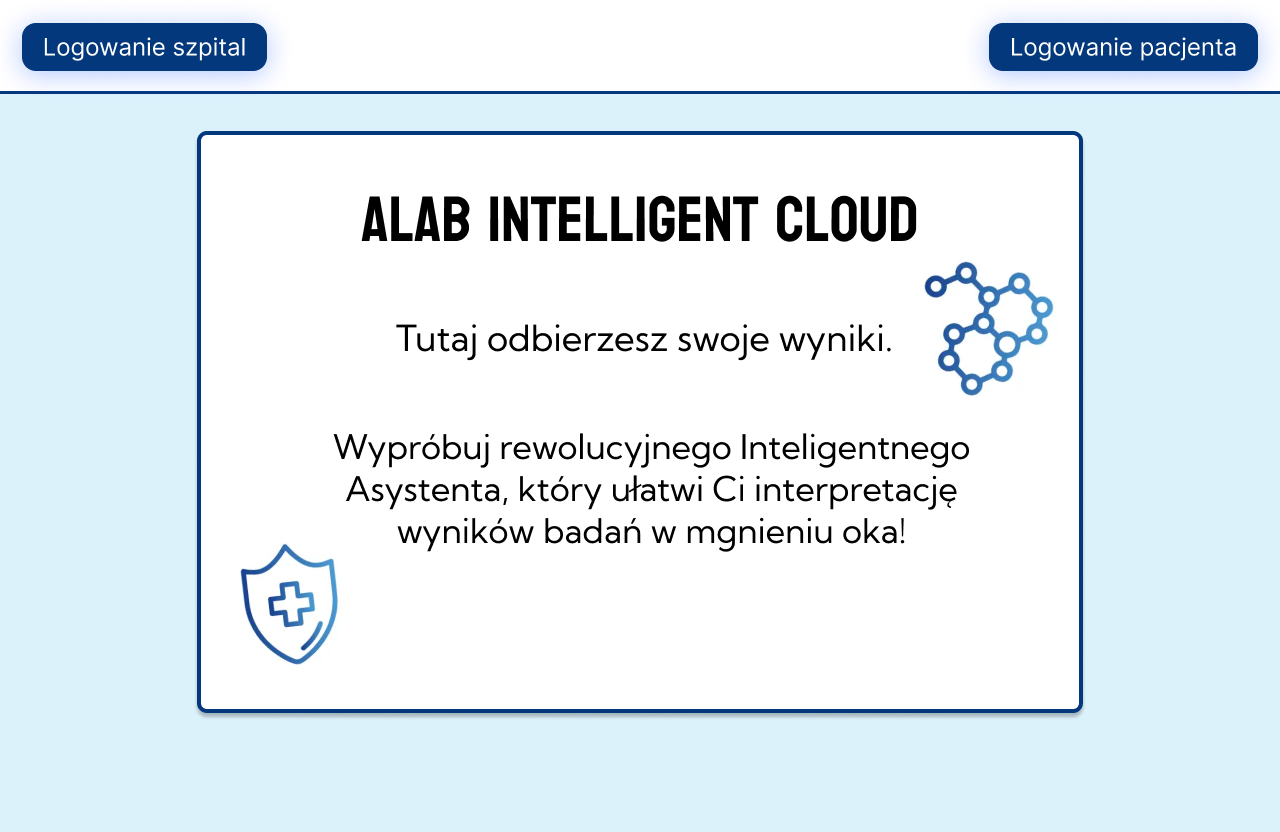
\includegraphics[width=0.8\textwidth]{landing page.png}
    \caption{Strona główna systemu\label{fig:mainPage}}
\end{figure}

W lewym górnym rogu znajduje się przycisk prowadzący do logowania personelu medycznego.
Z kolei w prawym górnym rogu znajduje się przycisk prowadzący do logowania pacjenta.

%TODO sekcja na 2FA

\section{Pacjent}

W systemie ASSASSIN pacjent ma możliwość przeglądania swoich wyników badań.
Na tym się kończy jego rola w systemie.

\subsection{Tworzenie konta}

Tworzenie konta to nie jest odpowiedzialność pacjenta.
Konto jest tworzone przy pierwszym kontakcie pacjenta z systemem przez lekarza lub inny personel.
Zatem jeśli pacjent nie ma konta, powinien skontaktować się z lekarzem.
Przy tworzeniu konta personel medyczny powinien podać pacjentowi login i hasło.

\subsection{Logowanie}

Po wejściu na stronę główną systemu, pacjent powinien kliknąć przycisk \textit{Logowanie pacjenta}.
Powinien pojawić się wtedy formularz logowania.
Wygląd formularza logowania jest przedstawiony na schemacie \ref{fig:login}.

\begin{figure}[h]
    \centering
    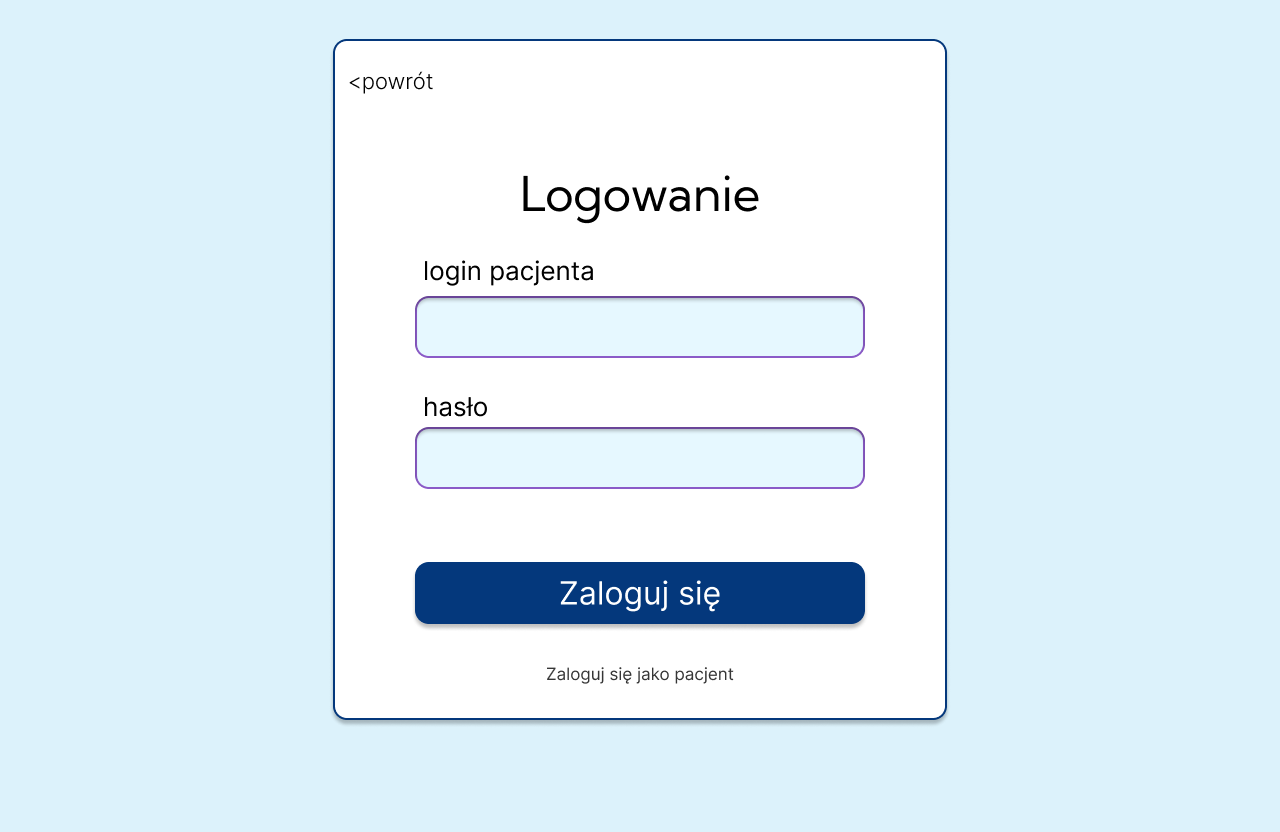
\includegraphics[width=0.8\textwidth]{logowanie.png}
    \caption{Widok logowania\label{fig:login}}
\end{figure}

Następnie pacjent powinien wpisać swój login i hasło, a następnie kliknąć przycisk \textit{Zaloguj się}.
W przypadku niepowodzenia, pacjent powinien skontaktować się z personelem medycznym w celu resetowania loginu i hasła.
Jeśli aktywowane jest logowanie dwuetapowe, pojawi się okno wpisywania kodu 2FA.
Przykładowy widok weryfikacji dwu stopniowej jest przedstawiony na schemacie \ref{fig:2FA}.

\begin{figure}[h]
    \centering
    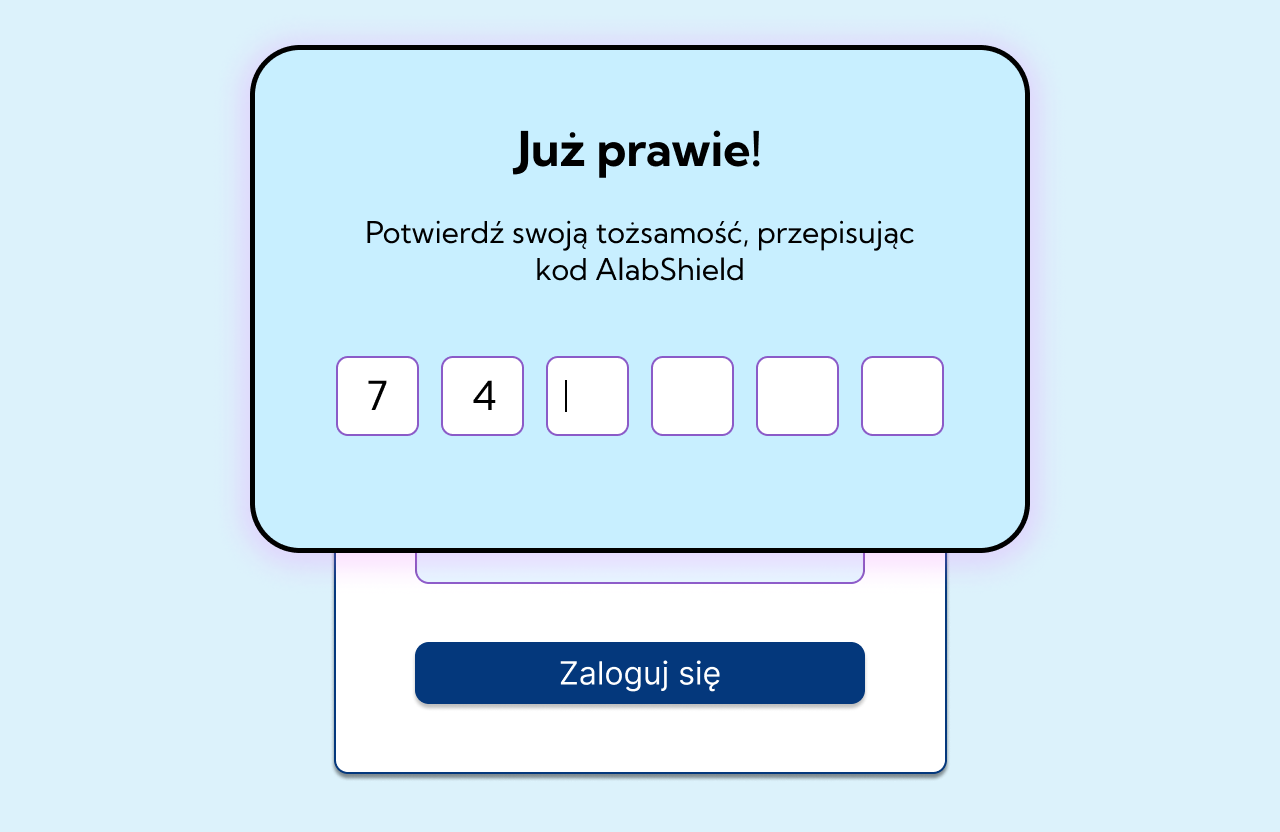
\includegraphics[width=0.8\textwidth]{2FA on log.png}
    \caption{Widok weryfikacji dwu stopniowej\label{fig:2FA}}
\end{figure}

Po wpisaniu kodu proces autentykacji jest zakończony i pacjent powinien zostać zabrany do strony profilowej.
Ze strony profilowej pacjent powinien mieć możliwość przejścia do strony z wynikami badań.
Strona profilowa jest przedstawiona na schemacie \ref{fig:patientProfile}.

\begin{figure}[h]
    \centering
    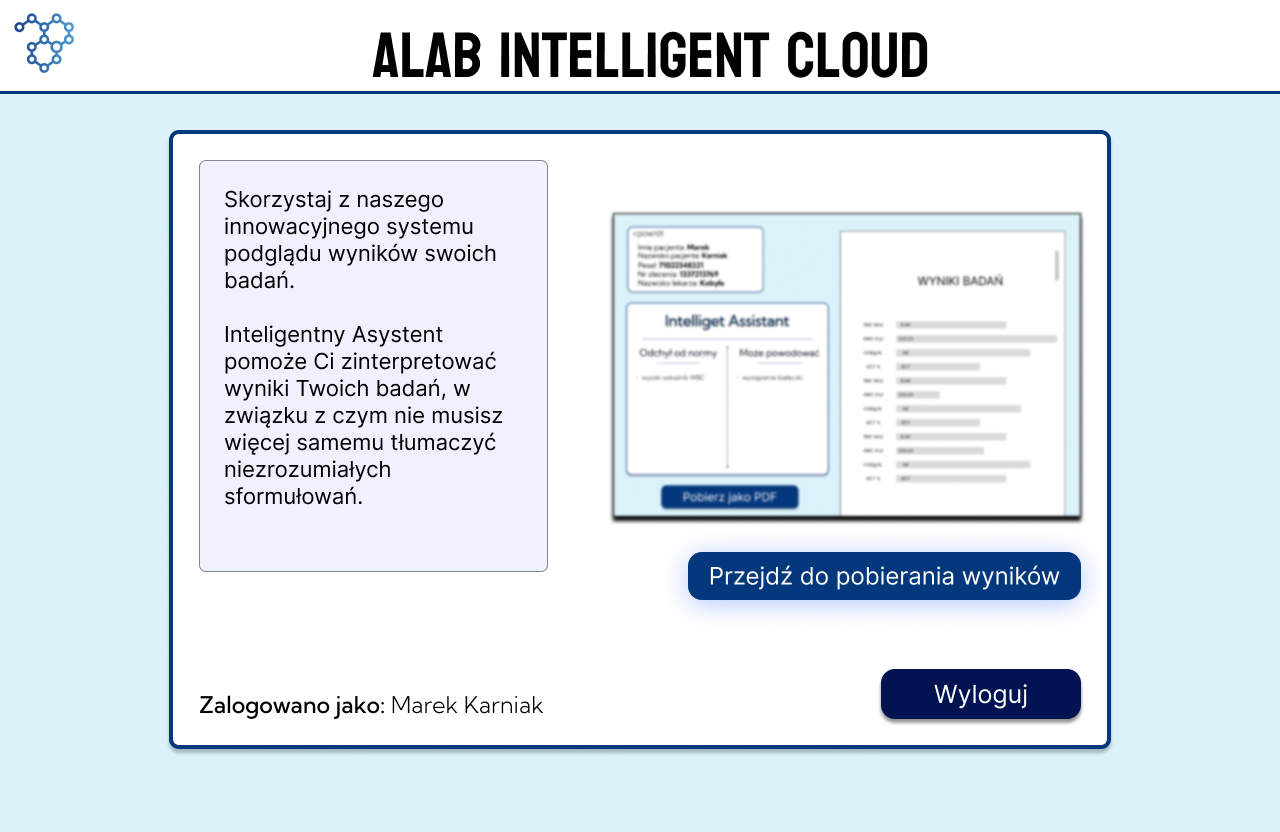
\includegraphics[width=0.8\textwidth]{logged in.png}
    \caption{Widok profilu pacjenta\label{fig:patientProfile}}
\end{figure}

\subsection{Odbieranie wyników}

Po kliknięciu na przycisk \textit{Przejdź do pobierania wyników} pacjent powinien zostać zabrany do widoku wprowadzania danych identyfikujących.
Widok wprowadzania danych identyfikujących badanie jest przedstawiony na schemacie \ref{fig:patientData}.

\begin{figure}[h]
    \centering
    \includegraphics[width=0.8\textwidth]{pobieranie-wyników.png}
    \caption{Widok pobierania wyników\label{fig:patientData}}
\end{figure}

Po wpisaniu informacji identyfikujących badanie pacjent powinien zostać zabrany do strony z wynikami.
Na stronie z wynikami z lewej strony powinien powinny pojawić się dwa panele: panel z informacjami o badaniu, oraz panel inteligentnego asystenta.
Z prawej strony powinien pojawić się panel z wynikami badań.
Widok wyników badań jest przedstawiony na schemacie \ref{fig:results}.

\begin{figure}[h]
    \centering
    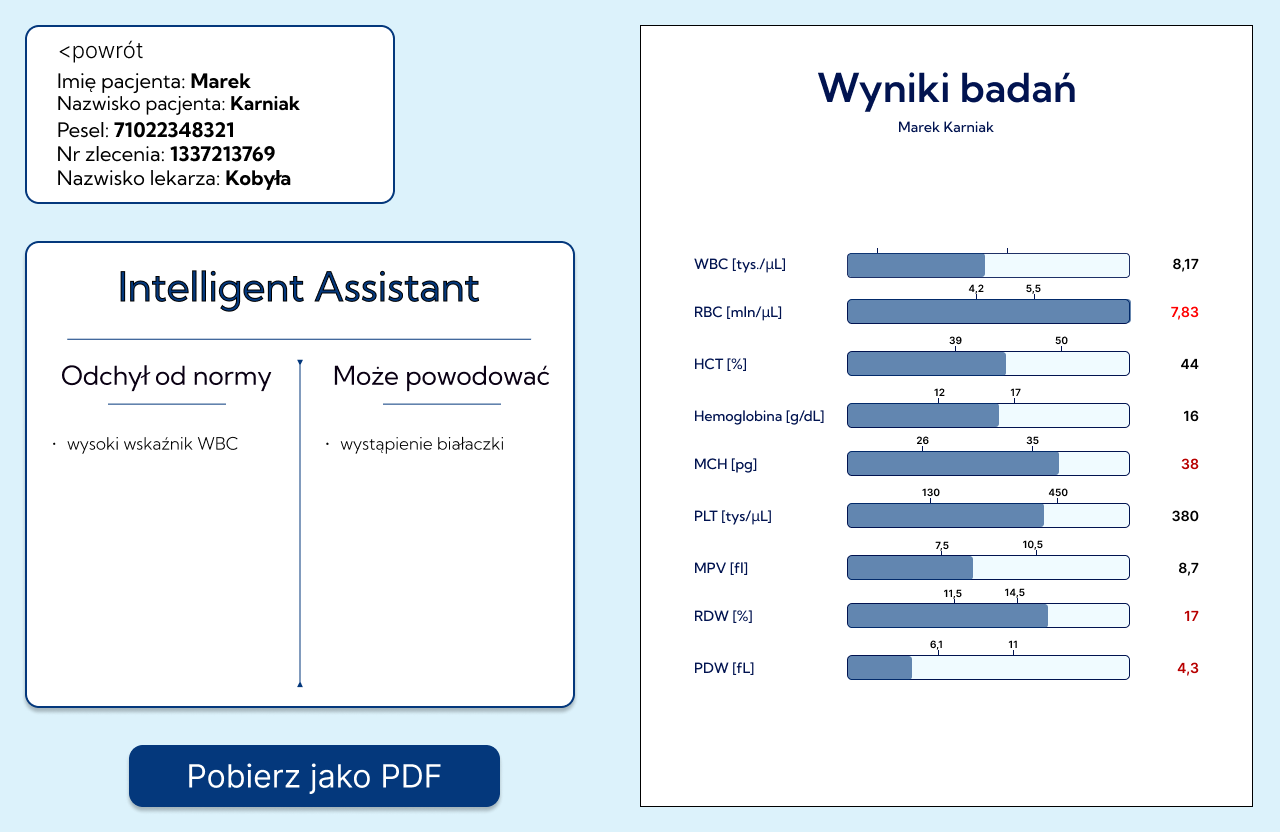
\includegraphics[width=0.8\textwidth]{wyniki-szpital.png}
    \caption{Widok pobierania wyników\label{fig:results}}
\end{figure}

Przez kliknięcie przycisku \textit{Pobierz} pacjent powinien pobrać plik z wynikami badań w postaci pliku PDF.

%TODO dodać opis lekarza



\end{document}